\chapter{Energy-based Multi-Modal Attention} 
\label{chapter-emma} 

In the Literature review (Chapter \ref{chapter-literature-review}) we concluded that previous work in multi-modal deep learning has been mostly focused on trying to increase the accuracy of the prediction. Few research has explicitly addressed the question of how using multiple modalities can improve the robustness. Inspired by how humans handle multiple senses robustly, I created a novel generic module that can easily be inserted into every trained multi-modal architecture. This chapter describes the ideas and architecture of the Energy-based Multi-Modal Attention module.

%----------------------------------------------------------------------------------------
%	SECTION 
%----------------------------------------------------------------------------------------

\section{Problem Statement}\label{sec:prob-statement}

We define the i.i.d. dataset $\mathcal{D}^{(N)}$ with $N$ samples  $(\mathbf{X},y)$. The input $\textbf{X}$ is composed of $M$ modes $\{\mathbf{x}_1, \ldots, \mathbf{x}_M\}$ of possibly different dimensions (e.g. images and sounds). The multi-modal network will be abbreviated as MMN. The model tries to make predictions $\hat{y}$ as close as possible to the groundtruth $y$ (see Figure \ref{fig:mnn}). The internal architecture of the MMN is often structured as a many-to-one encoder-decoder, where each encoder extracts features and the decoder is in charge of merging those together. Nonetheless, the EMMA module is not constrained to any specific MMN architecture.
\begin{figure}[!h]
\centering
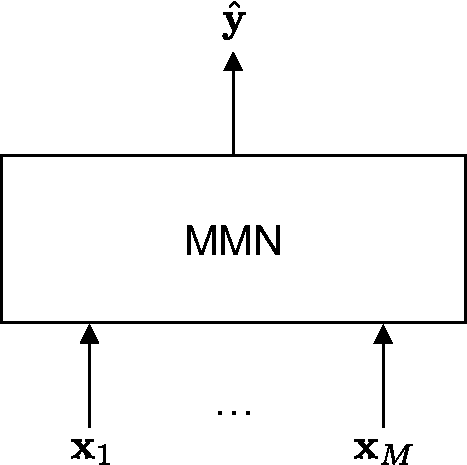
\includegraphics[scale=0.5]{figures/mlp-without-emma}
\caption{High-level view of a Multi-Modal Network}	
\label{fig:mnn}
\end{figure}

Current research in MMDL is mostly motivated by how to make use of the information gain of adding an extra mode to make better predictions. In this work, we want to leverage this same information gain to improve the robustness. We start from the assumption that for a sample where one mode $i$ is outlying, it is likely to find at least another mode $j$ who is not outlying. This permits us to think that if we find a way in that case to shift the attention from mode $i$ to mode $j$, the performance would be better off. This is done by computing an importance score $\alpha_i$ for each mode $i$ between zero and one, giving us the relative importance. The importance scores $\alpha_i$ are a measure of how valuable each mode $i$ is taking into account the outlyingness of all the modes. From those, we determine the attention scores $\beta_i$, representing the quantity of information that can pass through. Each mode is then multiplied by its respective attention score (see Figure \ref{fig:mnn-with-emma}). We justify later on why we do not directly multiply be the importance score instead. TODO: explain how missing values problem is implicitly solved
\begin{figure}[!h]
\centering
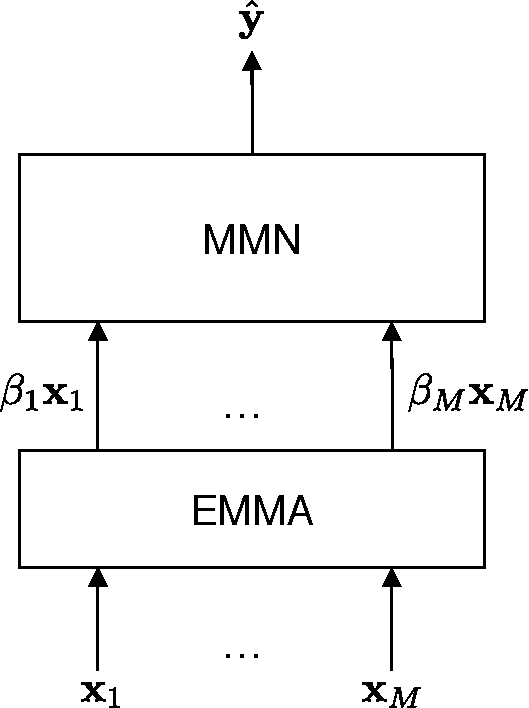
\includegraphics[scale=0.5]{figures/mlp-with-emma}
\caption[High-level view of a Multi-Modal Network \& EMMA]{High-level view of a Multi-Modal Network with the EMMA module}	
\label{fig:mnn-with-emma}
\end{figure}

There are two ways of interpreting this solution. First, EMMA can be seen as a sort of gate filtering perturbations out. Indeed, outlying modes can provoke high activations in the MMN, disturbing the predictions. But by masking the outlying modes we diminish those activations, making it easier for the MMN to make good preditions. Another way to view it, is to understand that the MMN model easily extracts $\beta_i$ and $\mathbf{x}_i$ from the multiplication. The model then learns to make more robust predictions based on the extra inputs $\beta_i$.

In Section \ref{sec:general-framework}  we describe the different steps along with their main objectives. Hereafter, each section will correspond to a specific step and will detail how it works. Next, the training of the module is explained along with some regularizers. The chapter ends with an enumeration of the main research questions that needs to be addressed in the experiments. 

%----------------------------------------------------------------------------------------
%	SECTION 
%----------------------------------------------------------------------------------------

\section{General Framework}\label{sec:general-framework}

As we just saw, the model needs to compute how important each mode is. To do this let us start by introducing three intrinsically tied properties describing the importance of a mode $i$:
\begin{itemize}
\item \textit{relevance}: how much does mode $i$ help improve the the accuracy?
\item \textit{outlyingness}: is the current sample much different from the training set? How much will it import the predictions?
\item \textit{coupling}: does mode $j$ has a strong influence on mode $i$? If so in which way? Does mode $i$ and $j$ carry complementary or redundant information?
\end{itemize}
We define the modal energy $E_i$ for a mode $i$ as an embedding of the three properties. Modal energies are constructed as learnable parametric functions of potential energies,
\begin{equation}
E_i = f(\Psi_i)  + \sum_{k\neq i}^M g[f(\Psi_i), f(\Psi_k)]
\label{eq:general-framework}
\end{equation}
The function $f$ is able to capture the relationship between relevance and outlyingness. Because $f$ is optimized with a loss on the predictions and is also a function of the potential $\Psi_i$. The role of the function $g$ is to learn the optimal coupling between modes. Modal energies are then normalized to the importance scores. Which is in some kind equivalent of going from a measure of absolute importance to one of relative importance.

Attention is viewed in psychology as a selection process between senses or more generally, modes. Deep Learning research regarding attention is in majority based on this view. In contrast, the famous economist and psychologist Daniel Kahneman sees attention as a shared resource with a limited capacity being allocated between the modes \citep{attention-is-effort}. We mimic the latter by slightly modifying a common attention function. This is done with the intention of improving the interpretability of EMMA (see Section \ref{sec:capacity}). In this work, we use attention to decide how much information of a certain mode will pass.

\begin{figure}[!ht]
\centering
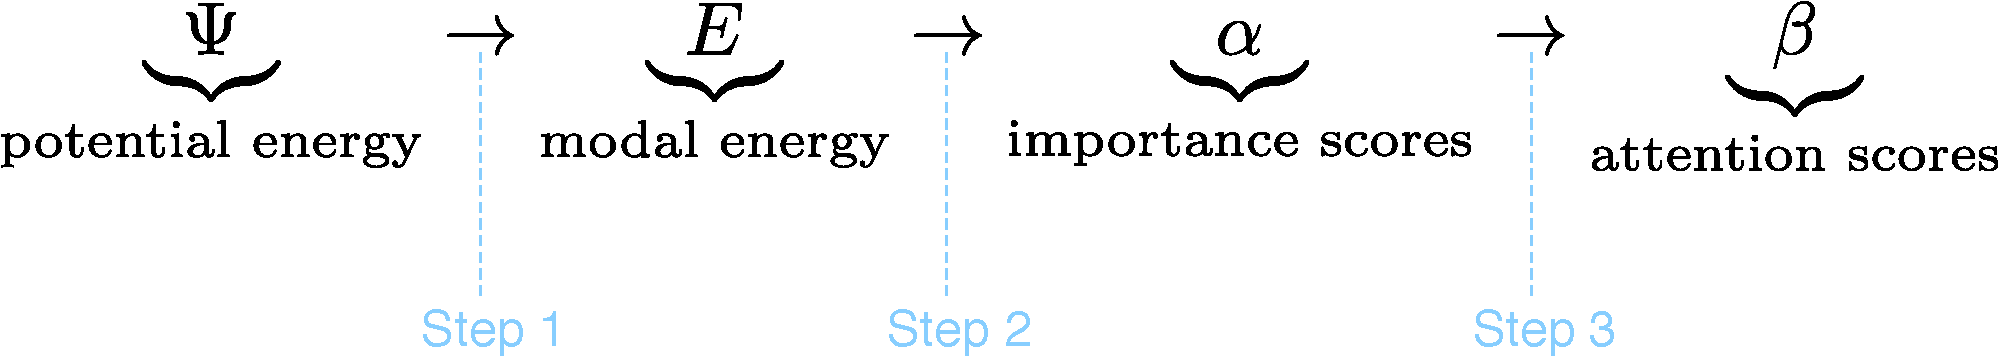
\includegraphics[scale=0.4]{figures/framework}
\caption[Summary of main steps in EMMA]{Summary of main steps in EMMA (step 2, 3 and 4 are detailed in the following sections, step 1 was explained in Chapter \ref{chapter-energy-estimation})}
\end{figure}

%----------------------------------------------------------------------------------------
%	SECTION 
%----------------------------------------------------------------------------------------

\section{From Potential to Modal energies (step 2)}
A problem overlooked so far is that we neglected the integration constant in the computation of the potential energy\footnote{Equation (\ref{eq:potential-prop})}. The potential can therefore take negative values. This is a problem because evaluating the gradient during the backpropagation involves taking a logarithm of $\Psi_i$\footnote{See Appendix \ref{chapter-misc}}, which is undefined for negative values. This problem is corrected by lowing the potential $\Psi_I$ to Euler's number $\mathrm{e}$ as
\begin{equation}
\Psi_i' = \max(\mathrm{e}, \Psi_i - \Psi_i^{(\text{min})} + \mathrm{e})
\end{equation}
With $\Psi_i^{(\text{min})}$ the lowest value of $\Psi_i$ in the training set. This correction avoids undefined values ($\Psi_i' \geq 0$) but also exploding gradient ($\Psi_i' \geq e$). The reason a max-operator is used is because lower energy values than $\Psi_i^{(\text{min})}$  can occur during inference.

The \textit{self-energy} of mode $i$ is defined as an energy capturing the outlyingness and the relevance of the mode. We write,
\begin{equation}
e_i = w_i\Psi_i' + b_i\,\,\, (=f(\Psi_i)), \qquad w_i, b_i \in \mathbb{R}^+
\end{equation}
The parameters $w_i$, $b_i$ are trained via a loss function on the predictions, thus adding the influence of the relevance. It also enables the model to face potentials on possibly very different scale, caused by the proportionality in Equation (\ref{eq:potential-prop}).

Furthermore, the \textit{shared energy} of mode $j$ on $i$ is constructed from the self-energies as follows
\begin{equation}
e_{ij} = w_{ij}e_i^{\gamma_{ij}}e_j^{1-\gamma_{ij}}\,\,\, (=g[f(\Psi_i), f(\Psi_k)]), \qquad w_{ij} \in \bigg[-\frac{1}{M-1}, +\frac{1}{M-1}\bigg],\,\, \gamma_{ij} \in [0,1]
\end{equation}
Adding the constraint $\gamma_{ij} = \gamma_{ji}$, the model can now discover the optimal coupling between the modes. It if learns a $\gamma_{ij}$ close to zero, mode $i$ and $j$ will influence each other much more than a $\gamma_{ij}$ near to one. The parameter $\gamma_{ij}$ learns the degree of coupling in the spectrum from strongly coupled ($\gamma_{ij}=0$) to independent ($\gamma_{ij} = 1$). The direction of coupling between mode $i$ and $j$ are learned by the weights $w_{ij}$ and $w_{ji}$. For a positive $w_{ij}$, an increase in self-energy $e_j$ causes an increase in $e_{ij}$. Whereas if $w_{ij}$ is negative, an increase in $e_j$ leads to a decrease in $e_{ij}$. The weights $w_{ij}$ are not imposed to be equal to $w_{ji}$, such that modes can influence each other asymmetrically. This assymetry is justified by the following example: a multi-modal problem with three modes A, B and C. Imagine the case where if mode A is missing, it is optimal that mode B takes over. But if B is missing it is optimal for C to take over. This can only be modelled with asymmetry.

Finally, the \textit{modal energy} of a mode is the sum of its self-energy and the shared energies with all the other modes:
\begin{equation}
E_i = e_i + \sum_{k\neq i}^M e_{ij}
\end{equation}
We can recognize Equation \ref{eq:general-framework}. This gives us also the \textit{total energy}, $E_{\text{total}} = \sum_i E_i$, offering an intuitive way to measure how uncertain the model is about its predictions.

%----------------------------------------------------------------------------------------
%	SECTION 
%----------------------------------------------------------------------------------------

\section{From Modal energies to Importance scores (step 3)}
The importance scores are computed from the modal energies via the Gibbs distribution:
\begin{equation}
\alpha_i = \frac{1}{Z}e^{-\rho E_i} \quad \text{with the partition function} \quad Z = \sum_{k=1}^M e^{-\rho E_k} 
\label{eq:gibbs-distrib}
\end{equation}
This guarantess the scores to be normalized and summing up to one. A mode $i$ will be said to be important if its score is close to one (low modal energy $E_i$). The hyperparameter $\rho$ represents the coldness, the inverse of the temperature. It controls the entropy of the importance scores distribution. At high temperature ($\rho \rightarrow 0$) the distribution becomes more uniform, and at low temperature ($\rho \rightarrow +\infty$) the importance scores corresponding to the lowest energy tends to 1, while the others approach 0 (see Figure \,\ref{fig:gibbs}). Careful tuning is thus necessary.

\begin{figure}[!h]
\centering
\begin{subfigure}{.5\textwidth}
  \centering
  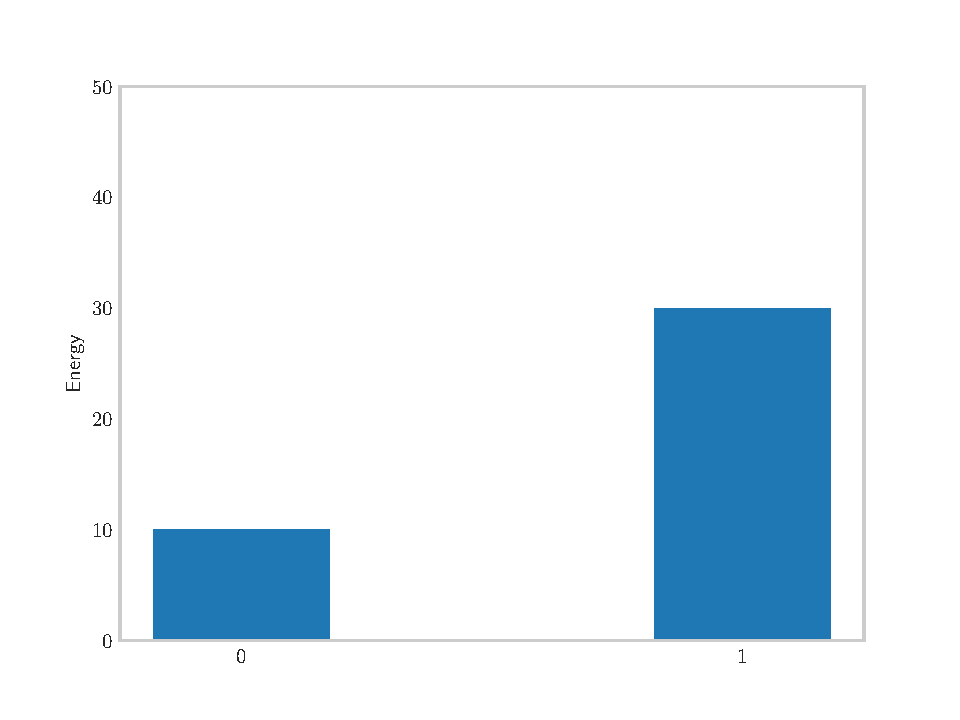
\includegraphics[width=.95\linewidth]{figures/input-gibbs}
  \caption{Energies}
\end{subfigure}%
\begin{subfigure}{.5\textwidth}
  \centering
  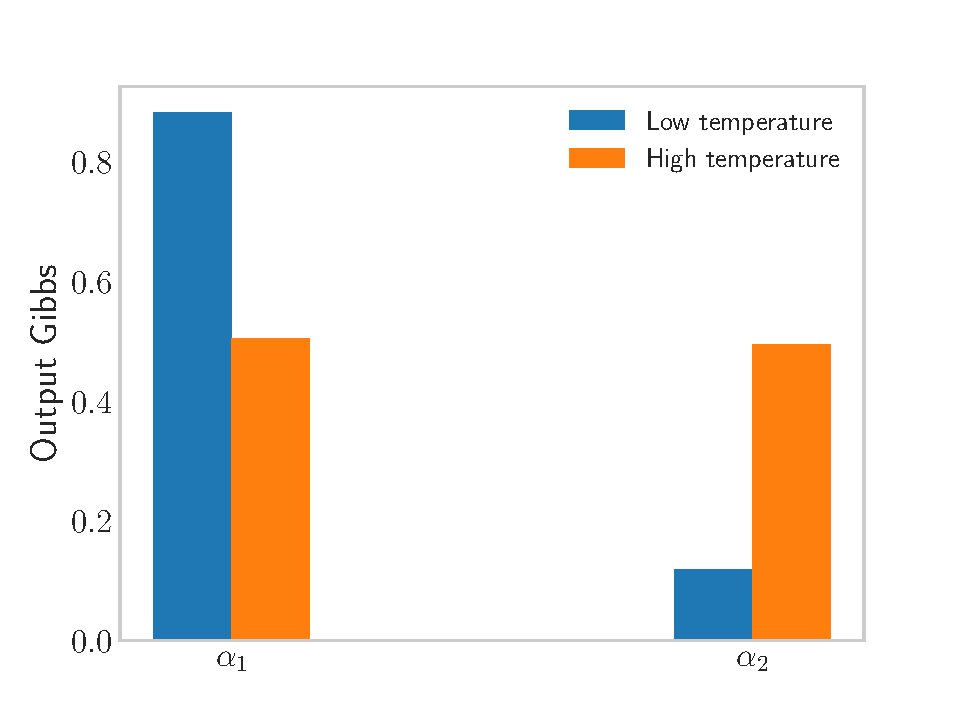
\includegraphics[width=.95\linewidth]{figures/result-gibbs}
  \caption{Importance scores}
\end{subfigure}
\caption[Input-output of Gibbs distribution for two different temperatures]{Input-output of Gibbs distribution for two different temperatures, low temperature ($\rho = 0.1$) and high temperature ($\rho = 0.001$)}
\label{fig:gibbs}
\end{figure}


%----------------------------------------------------------------------------------------
%	SECTION 
%----------------------------------------------------------------------------------------

\section{From Importance to Attention scores (step 4)}\label{sec:capacity}
The attention scores are given by
\begin{equation}
\beta_i = \tanh(g_a\alpha_i - b_a) \quad \text{with} \quad g_a > 0,\,\,b_a\in [0,1]
\end{equation}
The hyperbolic tangent adds non-linearity while the gain $g_a$ and bias $b_a$ permits the model to control the threshold and capacity (see Figure \ref{fig:attention-function}). The latter two concepts are detailed below.

\subsection*{Energy threshold}
The module will let information in mode $i$ pass by only if $g_a\alpha_i - b_a > 0$
\begin{equation}
\begin{split}
&\Leftrightarrow\log(\alpha_i) > \log(b_a/g_a)\\
&\Leftrightarrow E_i \geq \frac{\log(g_a/b_a) - \log(Z)}{\rho} = E_{\text{threshold}}
\end{split}
\end{equation}
where $E_{\text{threshold}}$ represents the maximal amount of energy a mode $i$ is allowed to have in order to pass. As be seen the gain and bias control the threshold. Nevertheless, the value of the partition function $Z$ makes the threshold dynamic. The partition function will be higher if the modes are more outlying, thus diminishing the thresholds. In other words, EMMA adapts the selectiveness with respect to the quality of the data. TODO: This can be linked more arousal \href{http://www.scholarpedia.org/article/Crossmodal_attention}{link}. Notice that the influence of the temperature ($\rho^{-1}$) is non-trivial to analyse, because $Z$ also depends on $\rho$.

\subsection*{Capacity}
There is nothing new about using an hyperbolic tangent as an attention mechanism. The difference however resides in how the linear combination is restricted. A very common attention function is written as $\tanh(\mathbf{W}\mathbf{\alpha}+\mathbf{b})$ whereas we have $\tanh(g_a\mathbf{I}\mathbf{\alpha}-b_a\mathbf{u})$ with $\mathbf{u}$ the unit vector $(1 \ldots 1)^T$. We argue the latter mimics better human's crossmodal attention. The capacity in psychology is viewed as the amount of resource that can be allocated. This can be translated in our case as,
\begin{equation}
\text{capacity} \triangleq \int_0^1 \tanh(g_a\alpha + b_a)d\alpha 
\end{equation}
Define the auxiliary variable $u = g_a\alpha + b_a$. Now using
\begin{equation}
\frac{du}{d\alpha} = g_a \Leftrightarrow d\alpha = \frac{1}{g_a}du
\end{equation}
we can write 
\begin{equation}
\begin{split}
\text{capacity} &= \frac{1}{g_a} \int_0^1 \tanh(u)du  \\
&= \frac{1}{g_a}\log[\cosh(g_a\alpha + b_a)]\bigg\rvert_{\alpha = 0}^1 + \cancel{\text{constant}} \\
&= \frac{1}{g_a}\log\bigg[\frac{\cosh(g_a + b_a)}{\cosh(b_a)}\bigg]
\end{split}
\end{equation}
If the capacity is too low, there is no sufficient information passed to the MMN to make predictions and thus the accuracy drops. On the other hand, if the capacity is too high, too much perturbations will pass leading to bad performances. The module learns the optimal trade-off. Observe that the concept of capacity can also be applied to $\tanh(\mathbf{W}\mathbf{\alpha}+\mathbf{b})$. In that case, each mode would have a different capacity. This could make EMMA more expressive, but the importance scores would be less meaningful. Another advantage of having only one capacity is that it is easier to control. In the next section, we show a simple regularizer giving us some control on the capacity. The interest of doing this, is the idea that minimizing the capacity would allow to gain more robustness againts unseen situations at the cost of some accuracy. This regularizer is played along with in the experiments (see Chapter \ref{chapter-experiments}), giving us some interesting insight.

\begin{figure}[!h]
\centering
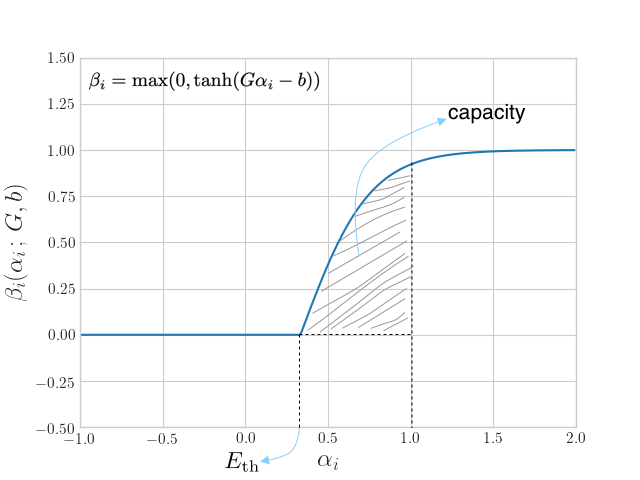
\includegraphics[scale=0.5]{figures/tanh-annotated}
\caption[Attention function]{Attention function, the max-operator generalizes the attention function to cases where $\alpha \in \mathbb{R}$}
\label{fig:attention-function}
\end{figure}
%----------------------------------------------------------------------------------------
%	SECTION 
%----------------------------------------------------------------------------------------

\section{Training \& Regularization}\label{sec:regul}
The end-to-end model (MMN \& EMMA) is trained in two phases (see Figure \ref{fig:training}). First, all the autoencoders are trained, one per mode. Once trained, the autoencoders are freezed. In the second phase, EMMA is inserted in front of the MMN and is trained end-to-end on both normal and corrupted data.

The motivation of EMMA is not only to improve predictions on the test-set. But also to see if it is able to handle new situations (robustness generalization) as expected. We also want EMMA to keep a certain level of interpretability. For those reasons we introduce two regularizers. The first one controls the capacity, where $\lambda_c$ can be positive/negative depending on if we want to maximize/minimize the capacity.
\begin{equation}
\tilde{\mathcal{L}} = \mathcal{L}(y,\hat{y}) + \lambda_c g_a - \lambda_e \Omega \quad \text{with} \quad \Omega = \sum_{k=1}^M \xi_k \log(\alpha_k) \quad \text{and} \quad \xi_k = \begin{cases}
      \xi_- = -1 & \text{if}\ \mathbf{x}_k\, \text{is corrupted} \\
      \xi_+ = +1 & \text{otherwise}
    \end{cases}
\label{eq:regularization}
\end{equation}
Additionally, regularizing the energy ($\lambda_e$) is done for interpretability purposes. If the parameters of modal energies are optimized only regarding the predictions ($\mathcal{L}$), we could have a large discrepancy between modal energies $E_i$ and their original potential energies $\Psi_i$. Although the energy regularizer is relatively straightforward, we will show below that some care needs to be taken.

\subsection*{Energy regularization}
Let $\theta = \{ \bm{\Gamma}, \mathbf{W}, \mathbf{b}\}$ be the set of all the parameters of step 2. The effect of the regularizer on this set of parameters with Gradient Descent is written
\begin{equation}
\theta' \leftarrow \theta + \epsilon\lambda_e\nabla_\theta\Omega
\label{eq:update}
\end{equation}
Remember the objective, we want this update to cause lower/higher modal energies $E_i$ for low/high potential energies. To verify this let us compute $\nabla_\theta\Omega$,
\begin{equation}
\nabla_{\theta} \Omega =\sum_{k=1}^M \xi_k \nabla_{\theta} \log(\alpha_k) 
\label{eq:dev}
\end{equation}
The gradient of the logarithm can be developed as
\begin{equation}
\begin{split}  
\nabla_{\theta}  \log(\alpha_k) &= \nabla_{\theta} \log \bigg[ \frac{e^{-\rho E_k}}{Z} \bigg] \\
&=  \nabla_{\theta}(-\rho E_k) -  \nabla_{\theta} \log \sum_{l=1}^M e^{-\rho E_l} \\
&=  -\rho \nabla_{\theta}E_k - \frac{\sum_{l=1}^M \nabla_{\theta} e^{-\rho E_l}}{\sum_{l=1}^M e^{-\rho E_l}} \\
&= -\rho \nabla_{\theta}E_k + \rho \frac{\sum_{l=1}^M e^{-\rho E_l} \nabla_{\theta}E_l}{\sum_{l=1}^M e^{-\rho E_l}} \\
&= \rho \Bigg[ -\big(1 - \frac{e^{-\rho E_k}}{Z}\big)\nabla_{\theta}E_k + \sum_{l \neq k}^M \frac{e^{-\rho E_l}}{Z} \nabla_{\theta}E_l \Bigg] \\
&= \rho \Bigg[ -\big(1 - \alpha_k\big)\nabla_{\theta}E_k + \sum_{l \neq k}^M \alpha_l \nabla_{\theta}E_l \Bigg] \\
\end{split}
\label{eq:grad-log}
\end{equation}
We go further by expressing the equation above with respect to the subset of parameters $\theta_i = \{[\gamma_{ik}, w_{ik}]_{k=1}^M, w_i, b_i\}$:
\begin{equation}
\nabla_{\theta_i}  \log(\alpha_k) = \begin{cases}
      -\rho(1-\alpha_i)\nabla_{\theta_i}E_i, & \text{if}\, i = k \\
       \rho\alpha_i\nabla_{\theta_i}E_i, & \text{if}\, i \neq k
    \end{cases}
\label{eq:log-split}
\end{equation}

The gradient of the regularizer can now be computed by plugging Equation (\ref{eq:log-split}) into the summation (\ref{eq:dev}). Let $M'$ be the number of uncorrupted modes. We obtain for an uncorrupted mode $i$,
\begin{equation}
\nabla_{\theta_i}\Omega = \xi_+\big[ -\rho(1-\alpha_i)\nabla_{\theta_i}E_i \big] + \big[(M'-1)\xi_+ + (M-M')\xi_-\big]\alpha_i\rho\nabla_{\theta_i}E_i
\label{eq:normal-exp}
\end{equation}
and for a corrupted mode $i$,
\begin{equation}
\nabla_{\theta_i}\Omega =\xi_-\big[ -\rho(1-\alpha_i)\nabla_{\theta_i}E_i \big] + \big[M'\xi_+ + (M-M'-1)\xi_-\big]\alpha_i\rho\nabla_{\theta_i}E_i
\label{eq:abnormal-exp}
\end{equation}
Substituting $\xi_k$, we can summarize Equations (\ref{eq:normal-exp}) and (\ref{eq:abnormal-exp}) as
\begin{equation}
\boxed{\nabla_{\theta_i}\Omega = -\big[(M-2M')\alpha_i + \xi_i\big]\rho\nabla_{\theta_i}E_i}
\end{equation}


Adding the constraint that $M' = \lfloor \frac{M+1}{2} \rfloor$, two cases can be distinguished. If the total number of modes $M$ is even, then we have
\begin{equation}
\theta_i' \leftarrow \theta_i - \epsilon\lambda_e\rho\xi_i\nabla_{\theta_i}E_i \quad \text{with} \quad \lambda_e \in \mathbb{R}^+
\end{equation}
Ignoring the second-order effects of the Taylor expansion, we can conclude from the equation above that the regularizer will update the parameters such that modal energies $E_i$ increase/decrease for corrupted/uncorrupted modes $i$.

In analogy, if M is uneven we have
\begin{equation}
\theta_i' \leftarrow \begin{cases}
       \theta_i - \epsilon\lambda_e\rho(1-\alpha_i)\nabla_{\theta_i}E_i, & \text{if $i$ is uncorrupted} \\
       \theta_i + \epsilon\lambda_e\rho(1+\alpha_i)\nabla_{\theta_i}E_i & \text{otherwise}
    \end{cases}
\end{equation}
The principle is the same as in the even case with an additional effect: the correction will be proportional to the error. High energies that have to be low and low energies that have to be high will have stronger gradients than their counterparts. This is similar to the positive and negative phase in the optimization of Restricted Boltzmann Machines.

To conclude, let us notice that some undesired effects can appear if we do not add the constraint $M' = \lfloor \frac{M+1}{2} \rfloor$. As an illustration, take $M' = \lfloor \frac{M+1}{2} \rfloor + 1$, Equation (\ref{eq:update}) becomes
\begin{equation}
\theta_i' \leftarrow \theta_i - \epsilon\lambda_e\rho(\alpha_i + \xi_i)\nabla_{\theta_i}E_i
\end{equation}
which is unstable for uncorrupted modes leading to a collapse where all energies tend to decrease.

%----------------------------------------------------------------------------------------
%	SECTION 
%----------------------------------------------------------------------------------------

\section{Advantages}
Listed below are the advantages of using EMMA instead of standard data-augmentation techniques.
\begin{itemize}
\item The generic design of EMMA permits it to be easily added to any architecture of multi-modal network
\item The burden on the multi-modal network is reduced, it only has to learn to make good predictions from the received information
\item Interpretability is increased, notably the uncertainty on the predictions as we will see in Section \ref{chapter-experiments}
\end{itemize}

%----------------------------------------------------------------------------------------
%	SECTION 
%----------------------------------------------------------------------------------------

\section{Research questions}
\begin{itemize}
\item Does EMMA increase the robustness compared to data augmentation techniques?
\item Is the use of the two regularizers experimentally validated?
\item Is the end-to-end model more interpretable with EMMA?
\end{itemize}

\newpage
\null
\vfill
\begin{center}
\begin{figure}[!h]
\centering
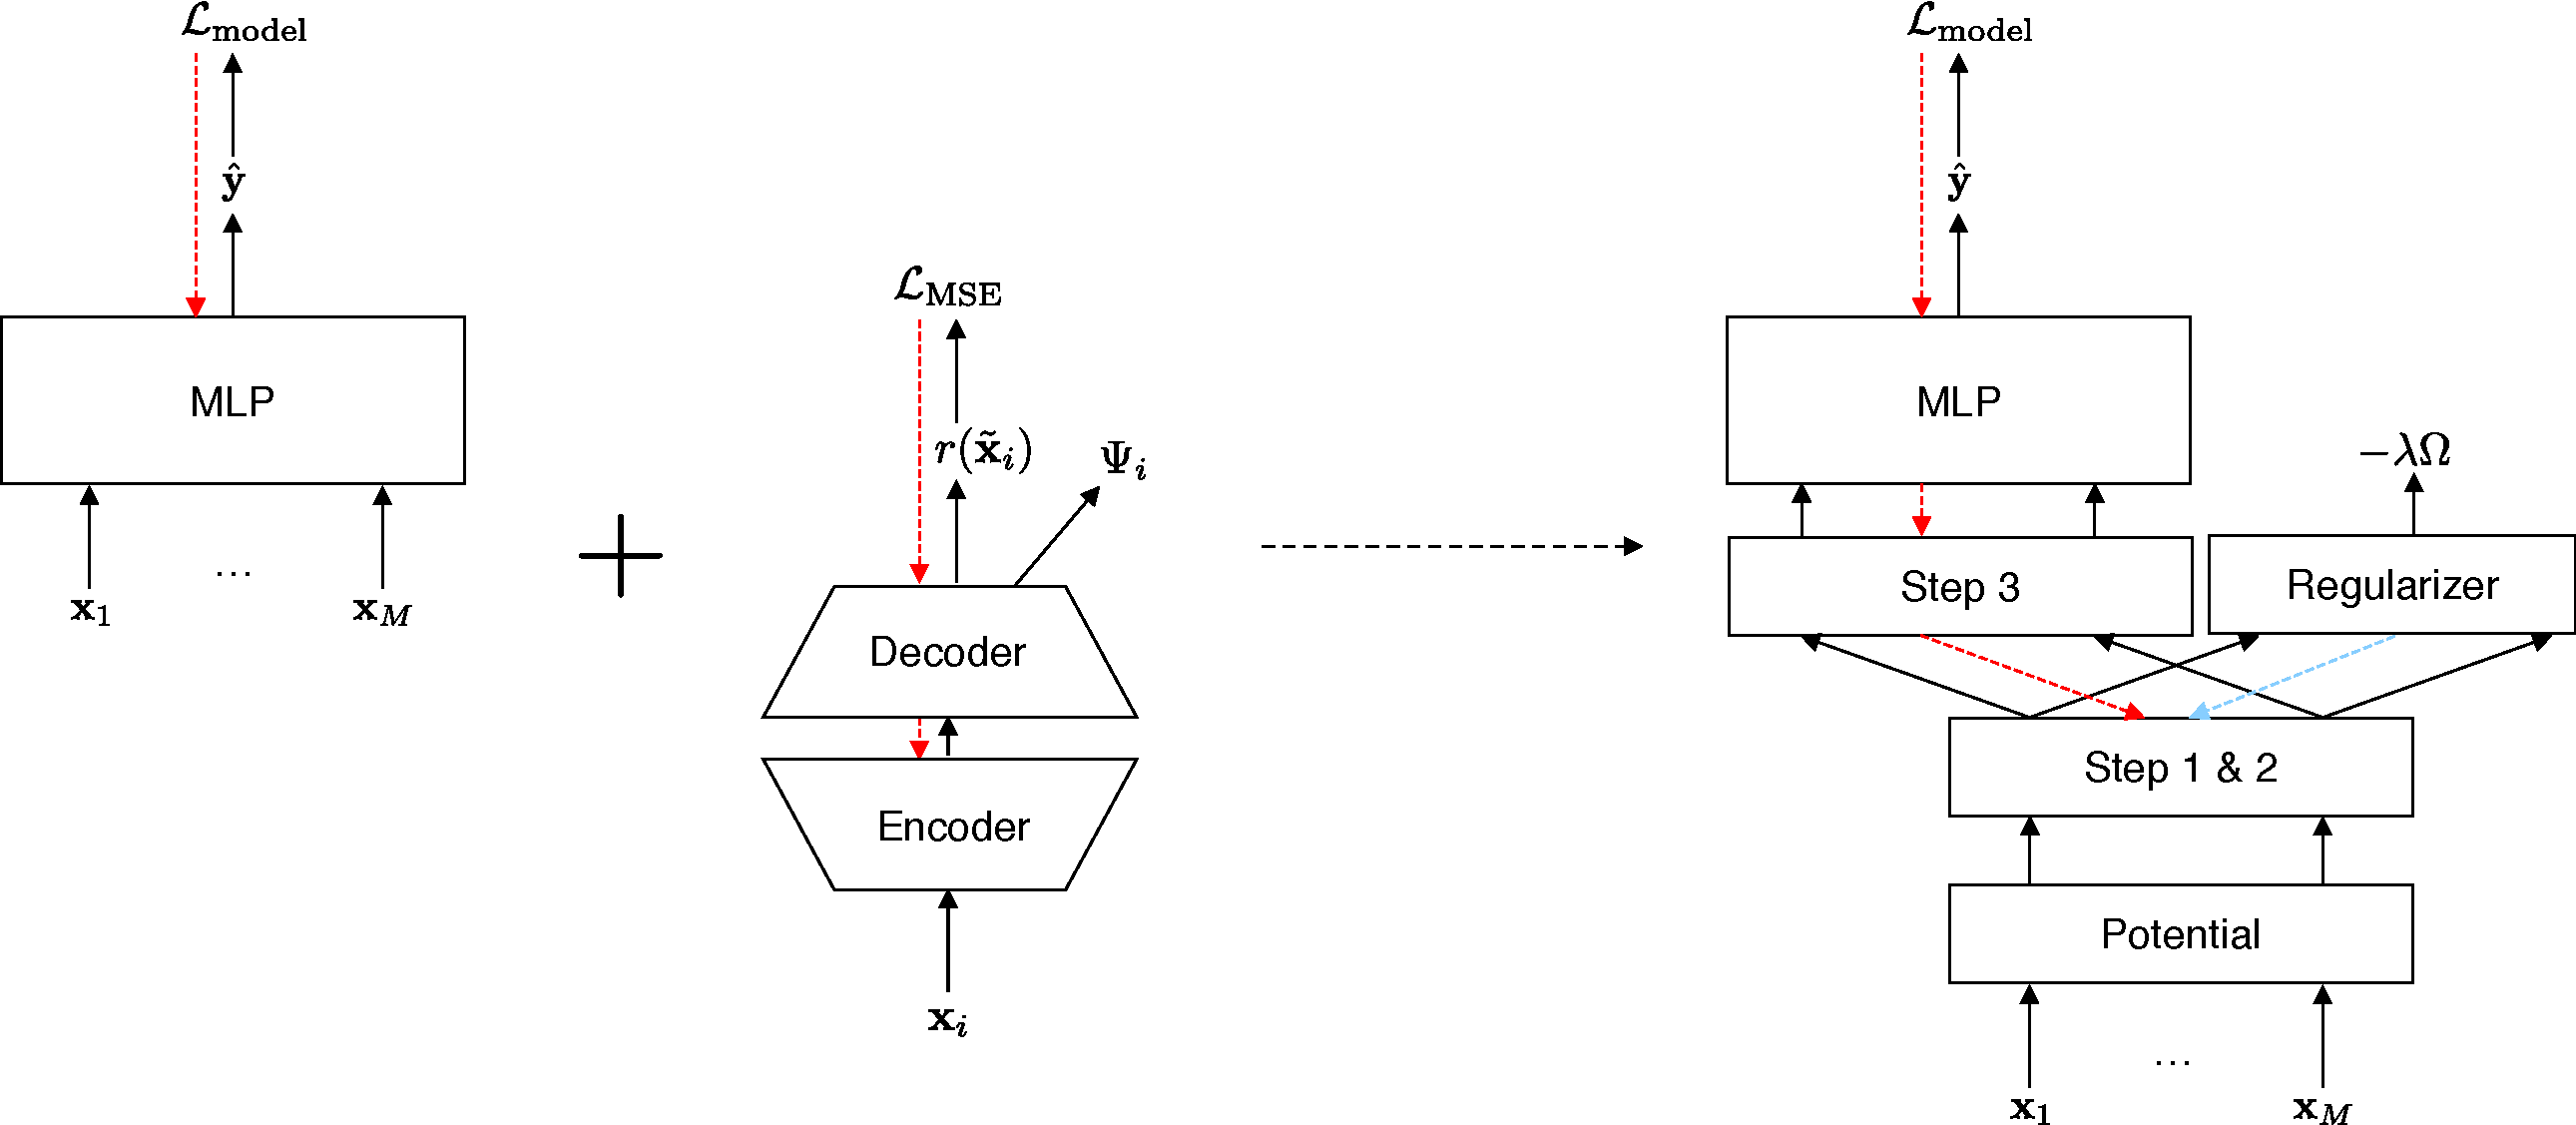
\includegraphics[scale=0.5]{figures/summary-training}
\caption{Summary of end-to-end training}	
\label{fig:training}
\end{figure}
\end{center}
\vfill
\clearpage